\chapter{Overview of Xtensa Instruction Set Architecture}

\section{Introduction}

Xtensa is a post-RISC ISA i.e it derives most of its features from RISC but also incorporates  certain features where CISC is advantageous. Xtensa has 24-bit instructions (few are even 16 bits!), unlike the conventional 32-bit instructions, to have code compactness \cite{leibson2006designing, tensilica2008whitepaper}.

\section{Registers}
\begin{description}[leftmargin=8em,style=nextline]
  \item[PC] Program Counter
  \item[AR] General purpose registers. In CPU configurations where window register option is enabled, there are 64 32-bit registers, 16 of which are  visible/accessible at a time. Without the window register option, there are 16 general purpose register.
  \item[SAR] Shift Amount Register. It is used to store the number of bits for subsequent shift instructions. Xtensa does not provide shift instructions which would have the shift amount specified in a general register (ar) operand.
  \item[PC] Holds the address of the instruction being executed.
\end{description}

\section{Windowed Register}

\underline{General purpose registers} (GPR) are used to store data temporarily for CPU while performing various operations. These registers are blazing fast but are limited in number (8 -- 32).

Typically, the number of registers present in the register file are equal to the registers directly accessible by the core. The Xtensa core can only access 16 GPR, namely a0 -- a15. So the register file contains 16 registers.

Xtensa also has a Windowed register option, which when enabled, extends this register file to contain 64 registers. Essentially, the register frame (a0 -- a15) acts as a window, through which only 16 registers are visible, that slides on this large register file having 64 registers. And hence the name: Windowed register.

Which 16 registers are visible is controlled by the WindowBase register. WindowBase register indicates where the window starts in the register file. Also, the shifting/rotation of this window occurs in units of 4. That means, the window starts at (WindowBase x 4)$^{th}$ position in the register file.

\begin{figure}[p]
    \center
    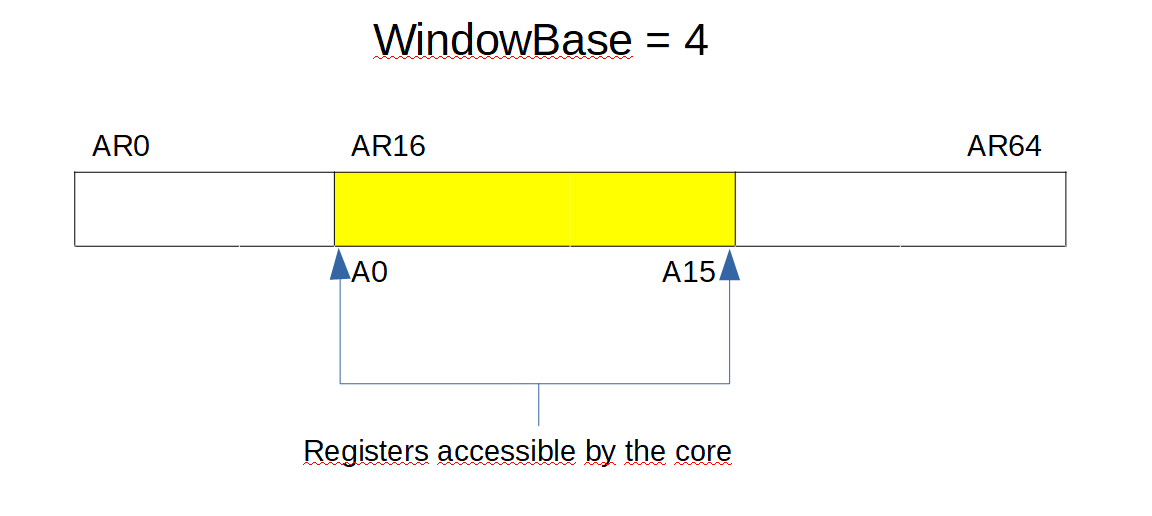
\includegraphics[width=0.9\textwidth]{Windowed_register.png}
    \caption{Register window}
    \label{fig:register-window}
\end{figure}

\section{Calling convention}

 Xtensa supports two different application binary interfaces (ABI) which also includes the calling conventions.
 
1. Windowed register ABI

2. Call0 ABI

We will cover only Windowed register ABI.

\subsection{Windowed register calling convention}

Return address is stored in a0 and the stack pointer is store in a1

Arguments to the functions are passed in both, registers and memory (stack). The first six arguments are passed in the registers and remaining go on the stack.

As for return values, they are returned in registers beginning from a2 till a5. If there are more than 4 values to be returned, the caller passes a pointer which is then populated by callee with all the return values.

\begin{longtable}{|p{5cm}|p{5cm}|}
    \hline
    Register & Use \\
    \hline
    a0 & Return Address\\ \hline
    a1 & Stack Pointer\\ \hline
    a2-a7 & Incomig Arguments\\ \hline
\end{longtable}

In Xtensa, subroutine calls are initiated using CALLN and CALLXN instructions. N is the windowed register option that specifies the amount by which the register window needs to be rotated for the callee. N can take values from 0, 4, 8 and 12. (call0/callx0 does not follow windowed register convention so further explanation does not apply for N = 0)

What does “rotation of window for the callee” exactly mean ?

When a subroutine is called using callN/callxN, WindowBase register is incremented by (N/4), so the registers visible when inside callee, through the window, would be different from caller because the register frame (a0 -- a15) would have moved.

In general, for a windowed register call callN/callxN:
aN of caller will be a0 of callee
a(N+1) of caller will be a1 of callee and so on.

So the caller needs to put the first argument of the callee in a(N+2), second in a(N+3) and so on.

While returning from the callee function, WindowBase register is decremented by (N/4) to keep the caller function registers same.

Let’s take an example:

\begin{verbatim}
/*
 * void bar(int x, int y);
 * 
 * void func(void)
 * {
 *     ...
 *     foo = bar(x, y);
 *     ...
 * }
 */

func:
    ...
    mov         a10, x    // a10 is bar’s a2
    mov         a11, y    // a11 is bar’s a3
    call8       bar
    mov         foo, a10  // a10 is bar’s a2 (return value)
    ...
\end{verbatim}

 When a function calls another function, it does not have to store its own arguments somewhere else to accomodate the arguments for the callee since the arguments of the callee is at a different physical location. The callee function internally will still use a2 to access its first argument but as you can see, a2 of the caller is at a different physical location than a2 of callee. If there was no windowing and the number of physical registers would be exactly 16 then a2 of caller and callee would be same. Thus for each function call, the data in these registers would have to be stored at some other memory location (stack) before calling any function and restore again after returning.

Accessing any memory location, other than register, is very slow and as a result this saving/restoring will have a negative impact on performance. So using windowed register convention saves us the overhead of such stores/restores and also reduces the code size.

\subsection{Stack Layout}

As mentioned, the stack pointer resides in a1 register. This stack pointer always points to the bottom of the stack!

Usually, function prologue sets up the stack for a function.

In Xtensa, ENTRY instruction is the function prologue

ENTRY instruction primarily does two things:
1. Allocates the stack frame for the function and sets the stack pointer.
2. Moves/rotates the register window by n as specified in the calln/callxn instruction.

Stack layout is always better explained through an illustration \ref{fig:window-abi-stack-layout}.

\begin{figure}[p]
    \center
    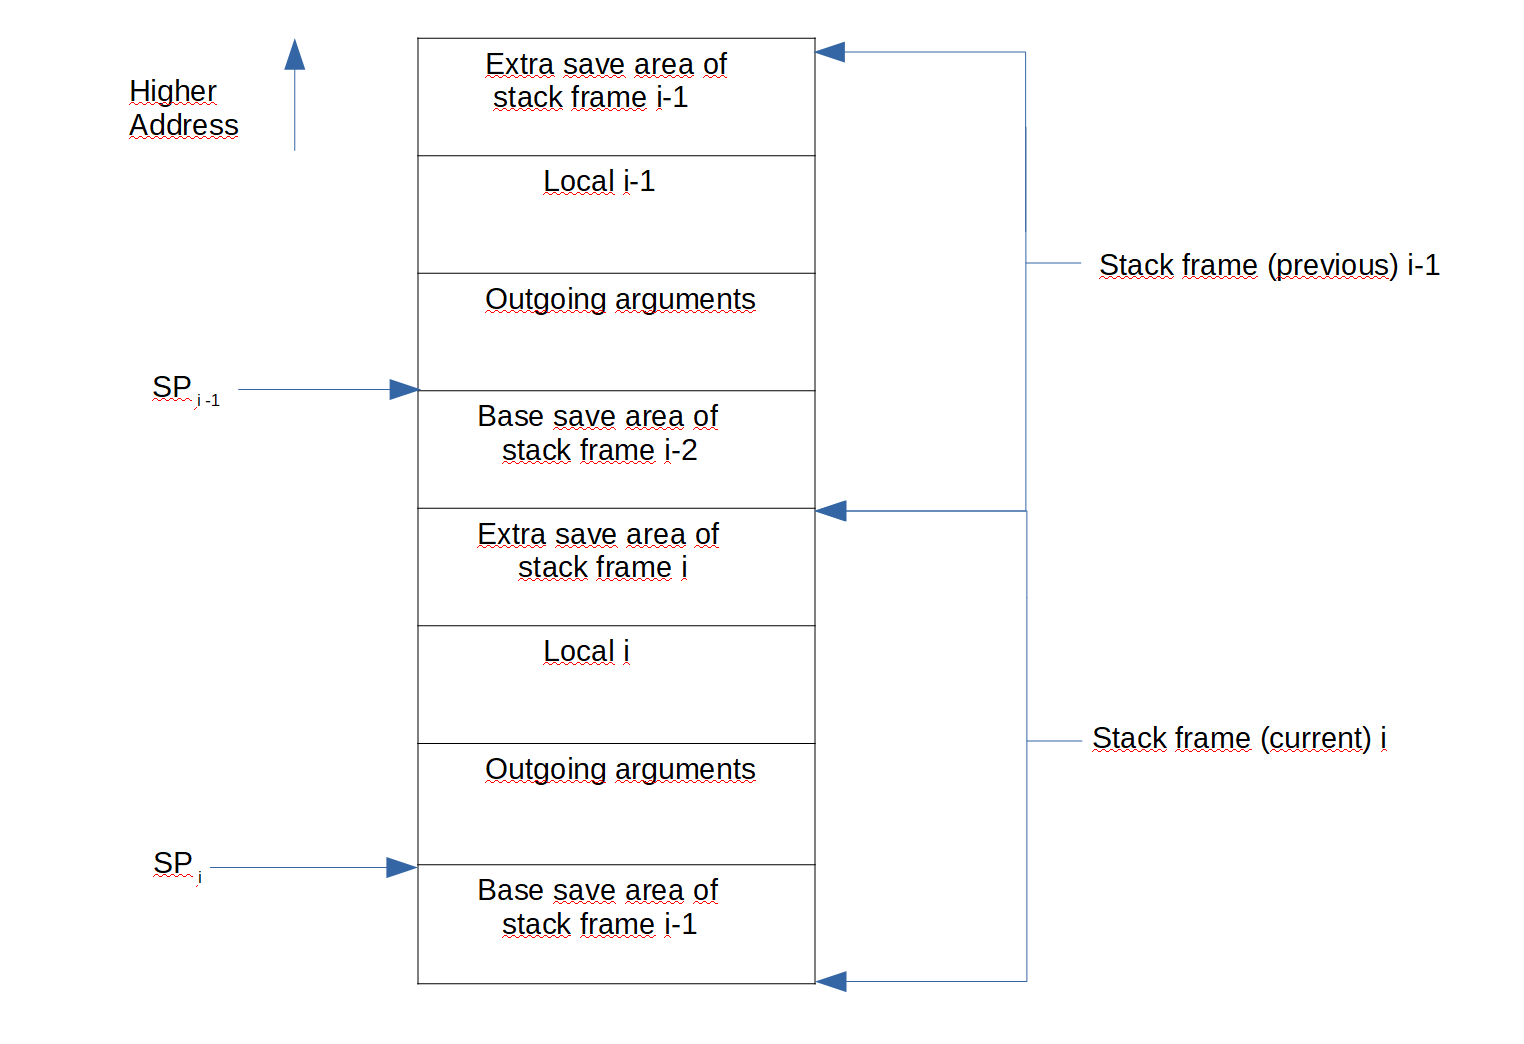
\includegraphics[width=0.9\textwidth]{Stack_layout.png}
    \caption{Windowed ABI stack layout}
    \label{fig:window-abi-stack-layout}
\end{figure}

For clarity, lets use sp as stack pointer instead of a1.

Like most architectures, in Xtensa too, stack grows downwards. If there are outgoing arguments, apart from the first 6 arguments, then they will go on the positive offset from sp. i.e 7th argument on sp, 8th on sp + 4 and so on. Above the outgoing arguments, local variables of that function are stored.

The region underneath the stack pointer, called Base Save Area, is of 16 bytes and reserved for saving the a0 -- a3 of the caller (previous frame) when the window overflow exception occurs. If more registers of the caller are required to be saved then it is stored in the Extra Save Area at the top of the caller (previous) stack frame. The location of saving registers of the caller (i-1) frame is highlighed in the image.

With all the necessary points covered, let’s take an example and connect all the dots.

Suppose, each function call is carried out using call8 and we start with WindowBase = 4

Function A calls B, B calls C, C calls D... till I, i.e:

\newcommand{\calls}{\textrightarrow{}}
\begin{longtable}{lc}
Functions&  A \calls B \calls C \calls D \calls E \calls F \calls G \calls H \calls I\\
WindowBase& 4 \calls 6 \calls 8 \calls 10 \calls 12 \calls 14 \calls 0 \calls 2 \calls 4\\
\end{longtable}
\let\calls\undefined

On each function call, the WindowBase will be incremented by 2 because call8 is used.

No. of bits in WindowBase register = $log_{2}$((No. of registers in register file)/4) = $log_{2}$(64⁄4) = 4. Thus the max value of WindowBase is 15.

As we have noticed, on the 9th function call the window wraps around to a point where the frame contains the data of a parent function, i.e a0,a1.. contains data of A. It implies that a8,a9.. of H are a0,a1.. of A.

A window overflow exception will be generated when H tries to modify a8,a9.. since it originally contains the context of A, so these must be saved to accommodate arguments of I. At this point, in the window overflow exception handler we must rotate the register window to frame A (WindowBase = 4).

a0 -- a3 are stored in the Base Save Area of B’s stack frame. B’s stack frame is accessible since a9 is a1 of B, which is B’s stack pointer.
a4 -- a7 are stored in the Extra Save Area of A’s stack frame.
Now whenever B returns, window underflow exception will be generated and we need to make sure that the corresponding exception handler would restore these values back into the registers.

